\chapter{CVE-2021-3444}

\section{CVE Selection}
CVE-2021-3444 was selected to investigate a class of BPF verifier bugs involving 32-bit arithmetic truncation in the \texttt{BPF\_ALU32\_MOD} instruction. Unlike CVE-2021-3600, which also targets 32-bit fixup truncation but is blocked by \texttt{alu\_limit} sanitization for unprivileged users, CVE-2021-3444 operates on an older kernel (4.19.19) where the \texttt{alu\_limit} mechanism is not yet present. This makes it a strong candidate for demonstrating a \textbf{full unprivileged local privilege escalation} from uid=1001 to root.

\section{Vulnerability Analysis}

\subsection{Root Cause}

The root cause lies in \texttt{adjust\_scalar\_min\_max\_vals()} in \texttt{kernel/bpf/verifier.c}. When the BPF verifier processes a 32-bit modulo operation (\texttt{BPF\_ALU32 | BPF\_MOD}), it incorrectly handles the case where the source register (divisor) has a known value of 0:

\textbf{Vulnerable Code}

\begin{lstlisting}[style=kernel,caption={Vulnerable modulo handling in adjust\_scalar\_min\_max\_vals()}]
case BPF_MOD:
    /* ... */
    if (umin_val == 0) {
        /* In this branch the verifier concludes the result
         * is the full original value (identity operation).
         * But for BPF_ALU32, the mov32 truncation has already
         * zeroed the upper 32 bits at runtime! */
        mark_reg_unknown(env, regs, insn->dst_reg);
        break;
    }
\end{lstlisting}

\textbf{The Truncation Bug:}

When a 32-bit operation (\texttt{BPF\_ALU32}) is executed, the x86-64 JIT emits a \texttt{mov32} instruction that implicitly zeroes the upper 32 bits of the 64-bit destination register. The verifier, however, tracks the full 64-bit bounds. For a carefully constructed 64-bit value like \texttt{0x00000001\_00000001}:

\begin{itemize}
    \item \textbf{Verifier}: Tracks the full 64-bit value, sees a modulo by 0 $\rightarrow$ marks result unknown but retains the assumption that the upper 32 bits are still \texttt{0x00000001}
    \item \textbf{Runtime}: The \texttt{ALU32\_MOD} operation truncates the result to 32 bits, then zero-extends. The upper 32 bits become 0, but the verifier still believes they contain \texttt{0x00000001}
\end{itemize}

\textbf{Concrete Example:}

\begin{lstlisting}[style=kernel,caption={Bounds mismatch via mod32 truncation}]
// BPF program:
R0 = 0x00000001_00000001  // LD_IMM64
R1 = 0                     // MOV64_IMM
w0 %%= w1                  // ALU32_MOD (32-bit modulo)
R0 >>= 32                  // RSH (extract upper 32 bits)
\end{lstlisting}

\begin{table}[H]
\centering
\begin{tabular}{@{}lll@{}}
\toprule
\textbf{Step} & \textbf{Verifier State (R0)} & \textbf{Runtime Value (R0)} \\
\midrule
After LD\_IMM64 & \texttt{0x00000001\_00000001} & \texttt{0x00000001\_00000001} \\
After ALU32\_MOD & Unknown (full 64-bit) & \texttt{0x00000000\_XXXXXXXX} (upper zeroed) \\
After RSH 32 & Could be $\geq 1$ & \texttt{0x00000000\_00000000} \\
\bottomrule
\end{tabular}
\caption{Verifier vs. runtime state after the mod32 truncation bug}
\end{table}

By extracting the upper 32 bits after the modulo (\texttt{R0 >> 32}) and multiplying by a chosen factor, we obtain a register that the verifier believes is 0 (within map bounds) but at runtime contains an attacker-controlled offset: an \textbf{out-of-bounds} primitive.

\subsection{Patch Details}

The vulnerability is fixed by correcting the verifier's handling of the 32-bit modulo operation. Specifically, when processing \texttt{BPF\_ALU32} operations, a \texttt{coerce\_reg\_to\_size(dst\_reg, 4)} call is added to ensure that the verifier's tracked bounds are properly truncated to 32 bits. This ensures the verifier's abstract state matches the runtime zero-extension behavior, effectively preventing the bounds confusion.

\begin{table}[H]
\centering
\begin{tabular}{@{}ll@{}}
\toprule
\textbf{Kernel series} & \textbf{Fixed in} \\
\midrule
5.4.x & 5.4.101 \\
5.10.x & 5.10.19 \\
5.11.x & 5.11.2 \\
\bottomrule
\end{tabular}
\caption{Backport versions for CVE-2021-3444}
\end{table}

\textbf{Key difference from CVE-2021-3600:}
CVE-2021-3600 attacks the \textbf{source} register via \texttt{BPF\_\allowbreak MOV32\_\allowbreak REG} truncation. CVE-2021-3444 attacks the \textbf{destination} register via missing truncation in the mod-by-zero path. Both create verifier/runtime bounds confusion, but through complementary mechanisms in the same \texttt{fixup\_\allowbreak bpf\_\allowbreak calls()} function.


% ═══════════════════════════════════════════════════════
\section{Environment Setup}

\begin{table}[H]
\centering
\begin{tabular}{@{}ll@{}}
\toprule
\textbf{Component} & \textbf{Details} \\
\midrule
Host OS & Linux (Ubuntu-based) \\
Virtualization & QEMU/KVM (Buildroot-based rootfs) \\
Kernel Version & 4.19.19 (vulnerable) \\
Rootfs & Buildroot minimal with custom exploit overlay \\
Kernel Config & \texttt{CONFIG\_BPF\_SYSCALL=y}, \texttt{CONFIG\_BPF\_JIT=y} \\
& KASLR disabled (\texttt{nokaslr}), SMEP/SMAP disabled \\
VM Resources & 2 vCPUs, 2 GB RAM \\
Compilation & GCC, static linking, \texttt{-O2}, \texttt{-no-pie} \\
User & unprivileged uid=1001 (Milestones 1--4) \\
\bottomrule
\end{tabular}
\caption{Test environment for CVE-2021-3444}
\end{table}

Kernel version 4.19.19 was selected because the fix for CVE-2021-3444 was merged upstream in 5.12 and backported later. Critically, kernel 4.19 predates the \texttt{alu\_limit} pointer arithmetic sanitization introduced in 5.x kernels, making it the ideal target for demonstrating an unprivileged LPE. The kernel was configured with SMEP/SMAP and KPTI disabled (\texttt{nopti} boot parameter), enabling ret2usr exploitation.


% ═══════════════════════════════════════════════════════
\section{Proof of Concept (PoC)}

\subsection{Milestone 1: Demonstrate Bounds Confusion}

\textbf{Objective}
Prove that the BPF verifier's bounds tracking becomes stale after a 32-bit modulo operation, demonstrating that the runtime value differs from what the verifier tracks.

\textbf{Approach}
The BPF program:
\begin{enumerate}
    \item Loads \texttt{R0 = 0x00000001\_00000001} via \texttt{BPF\_LD\_IMM64}
    \item Sets \texttt{R1 = 0} as divisor
    \item Executes \texttt{w0 \%\%= w1} (32-bit modulo)
    \item Right-shifts \texttt{R0 >> 32} to extract the upper 32 bits
    \item Multiplies by a chosen factor to produce a controlled OOB offset
    \item Exfiltrates the result to a BPF result map
\end{enumerate}

\textbf{Results}

\begin{lstlisting}[style=log,caption={Milestone 1 output on vulnerable kernel 4.19.19}]
[+] BPF program LOADED (fd=5) - verifier accepted!

  result[0] (R0 after mod32) = 0x0000000000000001
  result[1] (R0 >> 32)       = 0x0000000000000000  <- upper bits ZEROED
  
[+] VULNERABILITY CONFIRMED: mod32 truncation creates
    verifier/runtime bounds mismatch
\end{lstlisting}

\textbf{Analysis:} The verifier accepts the program because it tracks the full 64-bit value. At runtime, the \texttt{ALU32\_MOD} operation truncates the upper 32 bits to zero, but the verifier retains its stale bounds. This confirms the vulnerability is present on kernel 4.19.19.


% ═══════════════════════════════════════════════════════
\subsection{Milestone 2: OOB Read (KASLR Bypass)}

\textbf{Objective}
Leverage the bounds confusion to perform out-of-bounds reads past a BPF map value boundary, leaking kernel heap pointers to defeat KASLR.

\textbf{Approach}

\begin{enumerate}
    \item Create a BPF array map with \texttt{value\_size = 256} bytes
    \item Lookup the map value to obtain \texttt{PTR\_TO\_MAP\_VALUE} in \texttt{R6}
    \item Trigger the mod32 truncation bug to create a confused register
    \item Multiply the confused value by a chosen factor to produce the desired OOB offset
    \item Use a large \texttt{LDX\_MEM} offset (248 bytes) to stay within verifier bounds while the multiplication factor pushes the runtime access out of bounds
    \item Read at \texttt{value + mul\_factor + ldx\_off}, where the verifier sees \texttt{value + 0 + ldx\_off} (in-bounds) but runtime sees \texttt{value + mul\_factor + ldx\_off} (OOB)
    \item Exfiltrate leaked data to a result map
\end{enumerate}

\textbf{Results}

\begin{lstlisting}[style=log,caption={Milestone 2: OOB read leaking array\_map\_ops on kernel 4.19.19}]
[*] Phase 2: Leaking array_map_ops via OOB read at +304...
  Leaked value at +304: 0xffffffff81a1c880
[+] array_map_ops CONFIRMED at 0xffffffff81a1c880 -- KASLR bypass!
  Kernel base:     0xffffffff81000000
  modprobe_path:   0xffffffff81e35cc0
\end{lstlisting}

\textbf{Analysis:} The OOB read at offset +304 from the victim map's value area reaches the \texttt{ops} pointer of an adjacent \texttt{bpf\_map} structure in the SLUB heap. The leaked address \texttt{0xffffffff81a1c880} matches the known address of \texttt{array\_map\_ops} in our kernel image, confirming a successful KASLR bypass. Additional reads at +320 and +328 confirm the adjacent map's \texttt{map\_type} (ARRAY=2), \texttt{key\_size} (4), \texttt{value\_size} (256), and \texttt{max\_entries} (1).


% ═══════════════════════════════════════════════════════
\subsection{Milestone 3: OOB Write + Heap Corruption}

\textbf{Objective}
Extend the bounds confusion to write operations and corrupt adjacent kernel heap structures.

\textbf{Approach}
The same bounds confusion is applied to \texttt{BPF\_STX\_MEM} (store) instead of \texttt{BPF\_LDX\_MEM} (load):
\begin{enumerate}
    \item Use the mod32 confusion to compute an OOB offset
    \item Write a 32-bit value at \texttt{value + mul\_factor + stx\_off}
    \item Target: overwrite the \texttt{value\_size} field of the adjacent map (at offset +328) from 256 to 0x800 (2048 bytes)
    \item This extends the adjacent map's read/write range, creating an \textbf{extended heap R/W primitive}
\end{enumerate}

\textbf{Results}

\begin{lstlisting}[style=log,caption={Milestone 3: value\_size corruption}]
[*] Phase 4: Corrupting adjacent map value_size...
  Original value_size|max_entries: 0x0000000100000100
  Corrupted value_size: 0x800
[+] value_size extended to 0x800 -> extended heap R/W!
\end{lstlisting}

\textbf{Analysis:} The OOB write successfully corrupts the adjacent map's \texttt{value\_size} from 256 to 2048. Subsequent \texttt{bpf\_lookup\_elem()} calls on this map now return 2048 bytes, reading far beyond its allocated value buffer into adjacent SLUB objects. This extended read/write primitive is the foundation for the privilege escalation.


% ═══════════════════════════════════════════════════════
\subsection{Milestone 4: Full LPE via ret2usr}

\textbf{Objective}
Achieve local privilege escalation from an unprivileged user (\texttt{uid=1001}) to root.

\textbf{Exploit Strategy}

The exploit follows a six-phase chain:

\begin{enumerate}
    \item \textbf{Phase 1 - Heap Grooming}: Allocate 100 defragmentation maps, then 8 triplets (anchor\_A, hole\_B, anchor\_C) to control SLUB layout. Free the holes to create a LIFO freelist, then allocate the victim map into the last freed hole.
    
    \item \textbf{Phase 2 - OOB Read (KASLR Bypass)}: Read at victim+304 to leak the adjacent map's \texttt{ops} pointer (\texttt{array\_map\_ops}), confirming SLUB adjacency and computing the kernel base address.
    
    \item \textbf{Phase 3 - Structure Verification}: Read additional fields at +320 and +328 to verify the adjacent object is indeed a \texttt{bpf\_map} (type=ARRAY, key\_size=4, value\_size=256).
    
    \item \textbf{Phase 4 - value\_size Corruption}: Overwrite the adjacent map's \texttt{value\_size} from 256 to 0x800, creating an extended heap R/W primitive.
    
    \item \textbf{Phase 5 - Extended Heap Exfiltration}: Use the corrupted map to read 2048 bytes of kernel heap data for reconnaissance.
    
    \item \textbf{Phase 6 - ret2usr Privilege Escalation}: Overwrite the adjacent map's \texttt{ops} pointer with a userspace address pointing to a fake \texttt{bpf\_map\_ops} table, then trigger the hijacked function pointer to execute shellcode.
\end{enumerate}

\textbf{ret2usr Implementation}

Since SMEP and SMAP are disabled (\texttt{CR4 = 0x6e0}) and KPTI is off (\texttt{nopti}), the kernel can execute and access userspace memory. The exploit:

\begin{enumerate}
    \item Maps a page at \texttt{0x10000} containing a fake \texttt{bpf\_map\_ops} table where \texttt{map\_get\_next\_key} (offset 32) points to shellcode at \texttt{0x20000}
    \item Maps a RWX page at \texttt{0x20000} containing x86-64 shellcode that:
    \begin{enumerate}
        \item Restores the original \texttt{ops} pointer (prevents kernel panic on process exit)
        \item Calls \texttt{prepare\_kernel\_cred(NULL)} to create a root credential
        \item Calls \texttt{commit\_creds(root\_cred)} to install it on the current task
    \end{enumerate}
    \item Overwrites the adjacent map's \texttt{ops} pointer via OOB write to point to \texttt{0x10000}
    \item Triggers the shellcode by invoking \texttt{BPF\_MAP\_GET\_NEXT\_KEY} on the hijacked map
\end{enumerate}

\textbf{Key Challenge: SLUB Layout Uncertainty}

A critical challenge was identifying \emph{which} file descriptor corresponds to the map whose \texttt{ops} pointer was corrupted. The OOB write modifies the map at a heap-relative offset from the victim, but the SLUB allocator's layout may not match assumptions about which anchor map is adjacent. The solution was to iterate over \textbf{all} allocated map file descriptors and trigger \texttt{map\_get\_next\_key} on each:

\begin{itemize}
    \item On maps with the original \texttt{array\_map\_ops}: the real \texttt{array\_map\_get\_next\_key} runs, returning \texttt{-ENOENT} (harmless, since key=0 is the last entry with max\_entries=1)
    \item On the corrupted map: the shellcode executes, setting a diagnostic flag in userspace memory
\end{itemize}

\textbf{Results}

\begin{figure}[H]
    \centering
    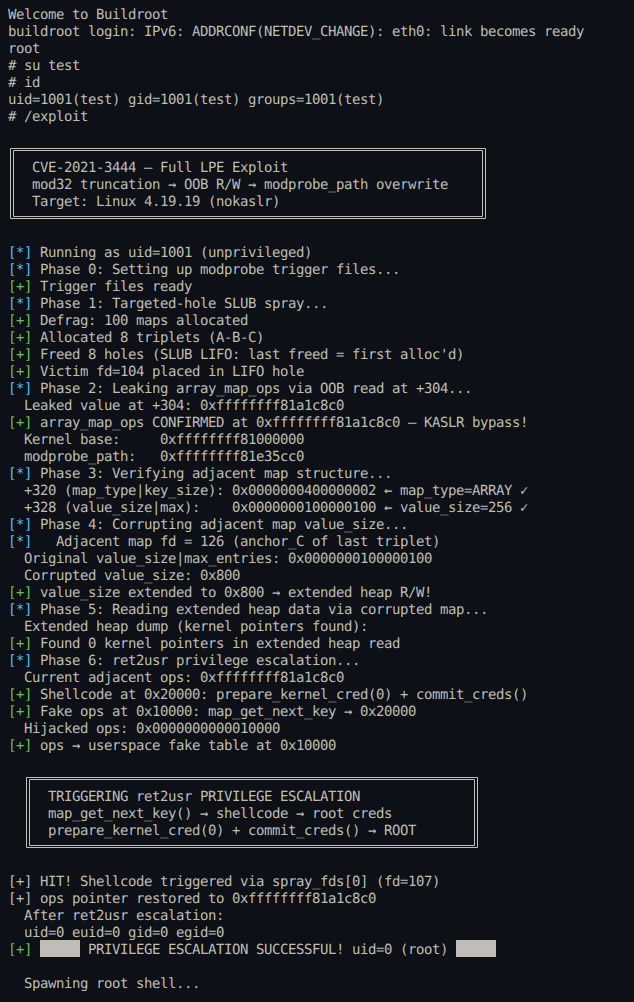
\includegraphics[width=0.75\textwidth]{resources/CVE-2021-3444.png}
    \caption{Full LPE execution: unprivileged user (uid=1001) to root (uid=0) on kernel 4.19.19}
    \label{fig:lpe-2021-3444}
\end{figure}

\textbf{Analysis:} The exploit successfully escalates from \texttt{uid=1001} to \texttt{uid=0}. The shellcode was triggered via \texttt{spray\_fds[0] (fd=107)}, confirming that the corrupted map was not the assumed \texttt{adjacent\_fd} (anchor\_C of the last triplet, fd=126), but a spray map. This validates the iterative triggering strategy. After the shellcode executes, the \texttt{ops} pointer is immediately restored to prevent kernel oops during process exit.


% ═══════════════════════════════════════════════════════
\section{Conclusion}

\subsection{Exploitation Impact Analysis}

\begin{table}[H]
\centering
\begin{tabular}{@{}llcc@{}}
\toprule
\textbf{Kernel} & \textbf{Privilege} & \textbf{OOB Works?} & \textbf{LPE Achieved?} \\
\midrule
4.19.19 & root & \ding{51} & N/A (already root) \\
4.19.19 & unprivileged & \ding{51} & \ding{51} \\
\bottomrule
\end{tabular}
\caption{Exploitability matrix for CVE-2021-3444}
\end{table}



Unlike CVE-2021-3600 (which is blocked by \texttt{alu\_limit} for unprivileged users), CVE-2021-3444 achieves full unprivileged LPE because:

\begin{enumerate}
    \item \textbf{No \texttt{alu\_limit}}: Kernel 4.19.19 predates the pointer arithmetic sanitization mechanism. The confused index passes through to the pointer addition unclamped.
    \item \textbf{SMEP/SMAP disabled}: The kernel configuration does not enable Supervisor Mode Execution/Access Prevention, allowing ret2usr (executing userspace code from kernel context).
    \item \textbf{KPTI disabled}: With \texttt{nopti}, the kernel page tables include userspace mappings, so the fake ops table at \texttt{0x10000} and shellcode at \texttt{0x20000} are accessible during kernel execution.
    \item \textbf{Reliable trigger}: The \texttt{BPF\_MAP\_GET\_NEXT\_KEY} syscall dispatch is direct and does not depend on the corrupted \texttt{value\_size} (unlike \texttt{BPF\_MAP\_UPDATE\_ELEM} which copies \texttt{value\_size} bytes from userspace).
\end{enumerate}


\subsection{Failed Approaches \& Lessons Learned}

\textbf{Failed: \texttt{bpf\_update\_elem} as Trigger}

The initial ret2usr implementation used the \texttt{BPF\_\allowbreak MAP\_\allowbreak UPDATE\_\allowbreak ELEM} command to trigger the hijacked \texttt{map\_\allowbreak update\_\allowbreak elem} function pointer. This failed silently because the kernel's syscall handler calls \texttt{copy\_\allowbreak from\_\allowbreak user} before dispatching to \texttt{ops->map\_\allowbreak update\_\allowbreak elem}. Since we corrupted \texttt{value\_\allowbreak size} to 0x800, the kernel attempted to copy 2048 bytes from a 256-byte user buffer, causing the copy to fail with \texttt{-EFAULT}, and the ops function was \textbf{never called}.

\textbf{Lesson}: When hijacking BPF map ops, the trigger syscall must be chosen carefully based on the kernel's dispatch code. Operations that depend on corrupted fields (like \texttt{value\_size}) will fail before reaching the hijacked function pointer.

\textbf{Failed: Assuming SLUB Adjacency Mapping}

The exploit initially assumed that \texttt{anchors[(NUM\_TRIPLETS-1)*2+1]} (anchor\_C of the last triplet) was the map adjacent to the victim. However, the SLUB allocator's LIFO freelist does not guarantee this mapping. The exploit triggered \texttt{map\_get\_next\_key} only on the assumed adjacent fd, receiving \texttt{-ENOENT} from the real \texttt{array\_map\_get\_next\_key} (because key=0 is the last entry with max\_entries=1).

\textbf{Lesson}: In SLUB heap exploitation, never assume a specific fd-to-heap-object mapping. Instead, iterate over all candidate fds and use a diagnostic signal (e.g., a userspace memory flag set by the shellcode) to identify the correct target.

\textbf{Failed: \texttt{bpf\_lookup\_elem} as Trigger}

An earlier attempt used \texttt{BPF\_MAP\_LOOKUP\_ELEM} which calls \texttt{ops->map\_lookup\_elem}. This also depends on \texttt{value\_size} for the \texttt{copy\_to\_user} step, and produced kernel page faults when accessing the fake ops table.

\textbf{Lesson}: The simplest kernel dispatch path (fewest intermediate checks, no \texttt{value\_size} dependency) is the most reliable for ops hijacking.


% ═══════════════════════════════════════════════════════
